% Chapter 4

\chapter{Synthesizing the Time-series Gene Expression Data to Enhance the Network Inference Performance Using the Autoencoder} % Main chapter title

\label{Chapter4} % For referencing the chapter elsewhere, use \ref{Chapter1} 

%----------------------------------------------------------------------------------------

% Define some commands to keep the formatting separated from the content 
% \newcommand{\keyword}[1]{\textbf{#1}}
% \newcommand{\tabhead}[1]{\textbf{#1}}
% \newcommand{\code}[1]{\texttt{#1}}
% \newcommand{\file}[1]{\texttt{\bfseries#1}}
% \newcommand{\option}[1]{\texttt{\itshape#1}}

%----------------------------------------------------------------------------------------

\section{Abstract}
It is a challenge to infer a gene regulatory network from the time-series gene expression data in the systems biology field. Lack of gene expression data samples is a factor limiting the performance of the inference methods. To resolve this problem, we propose a novel autoencoder-based approach that synthesizes virtual gene expression data to be used as input to the inference method. Through intensive experiments, we showed that using the synthetic gene expression as input improves the performance of the network inference method compared to that without it. In particular, the performance improvement was stable against the discretization level of gene expression, the number of time steps in the observed gene expression, and the number of genes.

%----------------------------------------------------------------------------------------

\section{Introduction}

GRNs describe the collective connections among genes and regulate their expressions. It is essential to clarify GRNs to understand the function and disease of organisms. Thus, the inference of GRNs has been an important research topic \parencite{Malvina2023}, and many diverse methodologies which are usually classified into model-free and model-based methods have been developed. In model-free approaches, gene interactions can be identified by various statistical and machine learning techniques including mutual information \parencite{Margolin2006, Yang2018, Liang2008}, random forests \parencite{HuynhThu2010, Petralia2015, Park2018}, or network deconvolution \parencite{Chen2014, SiegalGaskins2009}. In model-based methodologies, a quantitative dynamical model is employed to represent the system's dynamics such as the Boolean networks \parencite{Trinh2021, Hickman2009}, ordinary differential equation (ODE)\parencite{Ma2020, Li2011, Aalto2020, Bin2020}, regression method \parencite{Thorne2018, Michailidis2013, Breiman2001}, or dynamic Bayesian networks (DBN) \parencite{Murphy1999, Kim2003, Zou2005}.\par
In the model-based inference methods, it is necessary to optimize the model parameters by using gene expression data. It is obvious that the data from longer observation times would help infer GRNs more accurately. However, time series gene expression data is not always easily obtained \parencite{Murphy2002}. In some cases, it may be difficult to ensure that observations are made under the identical conditions throughout the observation period. Data augmentation has been considered as one of the effective approaches to resolve this data shortage problem. It has been frequently used in various domains such as image processing \parencite{Waqas2022, FridAdar2018, Zhang2023, Shin2018} and time series prediction \parencite{Forestier2017, Maweu2021, Leznik2021}. In the field of time series gene expression, several strategies have been also proposed to generate artificial data, in particular, through the Dialogue on Reverse Engineering Assessment and Methods (DREAM) challenge \parencite{Schaffter2011, DREAM2009}. Several previous investigations on this matter are accessible \parencite{Albert2008, deJong2002, DeJong2003, Mendes2003, VanDenBulcke2006}. These studies can generate simulated biological datasets that closely mimic real-world data, and provide researchers with tools to analyze and investigate genes. The Artificial Gene Networks (AGN) model is proposed to simulate temporal expression data for the identification of gene networks \parencite{MartinsLopes2011}. This model uses a feature selection technique where a specific gene remains constant, and the expression profiles of all other genes are observed. The goal is to identify a significant subset of predictors for the target gene. These studies proposed methods to produce synthetic data that closely resemble the real data. However, they have a limitation in producing a variety of data because they did not learn complex generation functions using data but tried to build simple rules. In particular, rule-based or manually designed simulations may fail to capture nonlinear or context-specific regulatory dynamics that naturally occur in biological systems. Additionally, these approaches often lack adaptability and may not generalize diverse datasets or unseen biological conditions. \par
In this study, we propose a network inference approach involving an autoencoder-based data generation model. For our problem, it is noteworthy that the autoencoder has some advantages over the generative adversarial network (GAN) \parencite{Goodfellow2020}. The autoencoder provides a simple yet effective framework with a lightweight architecture that enables stable training by optimizing a single objective. On the other hand, the GAN requires the simultaneous training of two competing networks which causes mode collapse, sensitivity to hyperparameters, and instability during training \parencite{Arjovsky2017, Salimans2016}. Thus, the autoencoder is more suitable for gene expression problems, where available datasets are typically small and heterogeneous. Several studies have shown that autoencoders perform well in low-data regimes and can effectively extract meaningful representations in biological applications \parencite{Tan2015, Chen2016}. In addition, the performance of autoencoders is less dependent on the underlying distribution of gene expression values, allowing better adaptability to biological variation. In this context, we utilize an autoencoder to learn a functional representation of gene expression dynamics from limited time-series data, generating additional synthetic samples to support more accurate network inference.
\section{Materials and Methods}

\subsection{Discretized Network Model}\label{sub:discretized}
In this study, we used a gene-wise discretized network model as presented in the previous study \parencite{Anh2023}. The discretized network can be modeled as a directed graph \( G(V, A) \), where the vertex set \( V = \{v_1, v_2, \dots, v_N\} \) corresponds to \( N \) genes, and edges \( A \subseteq V \times V \) encode regulatory interactions between them. The state of a gene \( v \) at time \( t \), denoted as \( v(t) \), assumes one of \( l \) discrete values from the set \( \{0, 1, 2, \dots, l - 1\} \). When \( l = 2 \) for all genes in \( V \), the network is referred to as a Boolean network \parencite{Kauffman1971}. Suppose that \( v \in V \) denotes a target node whose dynamics are governed by the interaction with \(k\) regulatory genes \( u_1, u_2, \dots, u_k \), where \( u_i \in V \). Let \( E \) and \( E_i \) denote the sets of possible discrete expression values for the gene \( v \) and the regulatory genes \( u_i \), respectively. The state of \( v \) at the next time step, \( v(t + 1) \), is determined by a discrete function \( f: E_1 \times E_2 \times \dots \times E_k \to E \), which maps the expression values of the \(k\) regulatory genes at time \( t \) to an updated state. Consequently, the update rule for \( v \) can be expressed as follows:
\[ v(t+1) = f(u_1(t), u_2(t), ..., u_k(t)). \tag{1} \label{eq: special}\] 

In this study, we adopted an update time lag of one. The total number of possible functions \( f \) is given by \( l^{\prod_i l_i} \), where \( l = |E| \) and \( l_i = |E_i| \) denote the cardinalities of the sets \( E \) and \( E_i \),~respectively.

\subsection{Network Inference Problem}
In this study, we addressed the problem of network inference from time-series gene expression data, aiming to recover both the regulatory interactions and their associated update functions. The quality of the inferred network was evaluated by comparing the trajectories it generates with those observed in the original time-series data. Let \({\bf v'}~=~[v'(1), v'(2),...,v'(T)]\) denote the sequence of the predicted expression states of gene \(v\) for a time step ranging from 1 to \(T\), based on the inferred discretized network. Then, the dynamic accuracy of the inferred network is defined as follows:
\[Dynamic Accuracy = \frac{1}{N \cdot T}\sum_{i=1}^{N}\sum_{t=1}^{T}(1-D({\bf{v', v}})), \tag{2} \label{eq:special}  \]
where \(T\) denotes the total number of time points and \(D({\bf{v', v}})\) is the Hamming distance between two sequences of \({\bf v'}\) and \({\bf v}\).

\subsection{Structural Performance Metrics}\label{sub:metrics}
{In this study, we employed three well-known evaluation metrics, namely precision, recall, and structural accuracy to quantify the structural similarity between the inferred and the corresponding ground truth networks. Precision measures the proportion of correctly inferred regulatory connections (\(TP\)) among all predicted ones (\(AP\)) and is defined as~follows:
\[Precision =\frac{TP}{AP}. \tag{3} \label{eq:special}\]
\indent Recall quantifies the proportion of correctly inferred connections (\(TP\)) over the whole number of connections (\(P\)) and is defined as~follows:
\[Recall =\frac{TP}{P}. \tag{4} \label{eq:special}\]
\indent Finally, structural accuracy assesses the proportion of true positive and negative predictions (\(TP\) and \(TN\)) out of all positive and negative connections (\(P\) and \(N\)) and is defined as~follows:
\[Structural Accuracy =\frac{TP + TN}{P+N}. \tag{5} \label{eq:structural}\]}


\subsection{Network Inference Method} \label{network_inference}
In this study, we synthesized time-series discrete expression data to improve the existing network inference method. To this end, we used mutual information based on multiple-level discretization network inference (MIDNI) \parencite{Anh2023}. The latter is an algorithm developed from the mutual information-based Boolean network inference method (MIBNI) \parencite{Barman2017}. The former reconstructs the discrete network by properly discretizing gene expression values into two or three levels depending on their distribution, whereas the latter infers the Boolean network based on the binarized gene expression values. This higher degree of freedom in expression led to more accurate inference results in MIDNI.

\subsection{Autoencoder Model}
The concept of an autoencoder was originally proposed by LeCun in 1987 \parencite{LeCun1987}. It is an artificial neural network designed to acquire efficient representations of input data, primarily for dimensionality reduction or feature extraction. It comprises two components, namely an encoder and a decoder. The encoder compresses the input data into a reduced-dimensional representation, referred to as the \enquote{latent space} or \enquote{code}, whereas the decoder utilizes the compressed latent representation to recreate the original input data with maximal fidelity. Since it was invented, numerous autoencoder variations have been effectively used in a variety of domains, including natural language processing \parencite{Li2015,Freitag2018,Akram2022}, computer vision \parencite{Zhou2023,Parmar2021,Cheng2018}, and speech recognition \parencite{Vachhani2017,Karita2019}. In our study, we employed a conventional autoencoder with a reasonable number of hidden layers to achieve a compromise between efficiency and training duration \parencite{Geron2022, Song2022}. Unlike traditional autoencoders that aim to reconstruct the input data itself, the proposed model is trained to predict the next state \( v(t+1) \) given the current state \( v(t) \) as input. This architecture retains the encoder--decoder structure, but the training objective shifts from input reconstruction to temporal state prediction. It seeks to reduce the discrepancy between the actual and predicted values by minimizing the loss function. By learning a compressed latent representation of \( v(t) \) that captures temporal dynamics, the decoder is optimized to generate the corresponding \( v(t+1) \) rather than reproducing \( v(t) \). {While the model may produce diverse gene expression profiles due to the limited dataset, this variation is consistent with natural biological variability. Instead of evaluating the biological plausibility of the synthetic data directly, we assess its utility through downstream network inference, interpreting the successful reconstruction of gene regulatory networks as an indirect yet meaningful indicator of data quality.}

\section{Our Proposed Method}
Figure~\ref{fig:chapter4_framework} shows the entire framework of our approach. An observed discrete gene expression dataset is given as an input. It is represented by a \(K\) $\times$ \(N\) discrete matrix, where \(K\) and \(N\) indicate the number of observed time steps and genes, respectively. The matrix is used to generate two other discrete matrices of \((K-1)\) $\times$ \(N\) size, which are input--target pair matrices. They establish a relationship between consecutive network states, which will be learned by the autoencoder. The learned autoencoder can synthesize gene expression values after the observed time steps. The synthesized and observed discretized gene expressions are combined into a single matrix, and this is used as input for the inference algorithm MIDNI. Each part of our approach is explained in detail in the next subsections.

\begin{figure}[th]
\centering
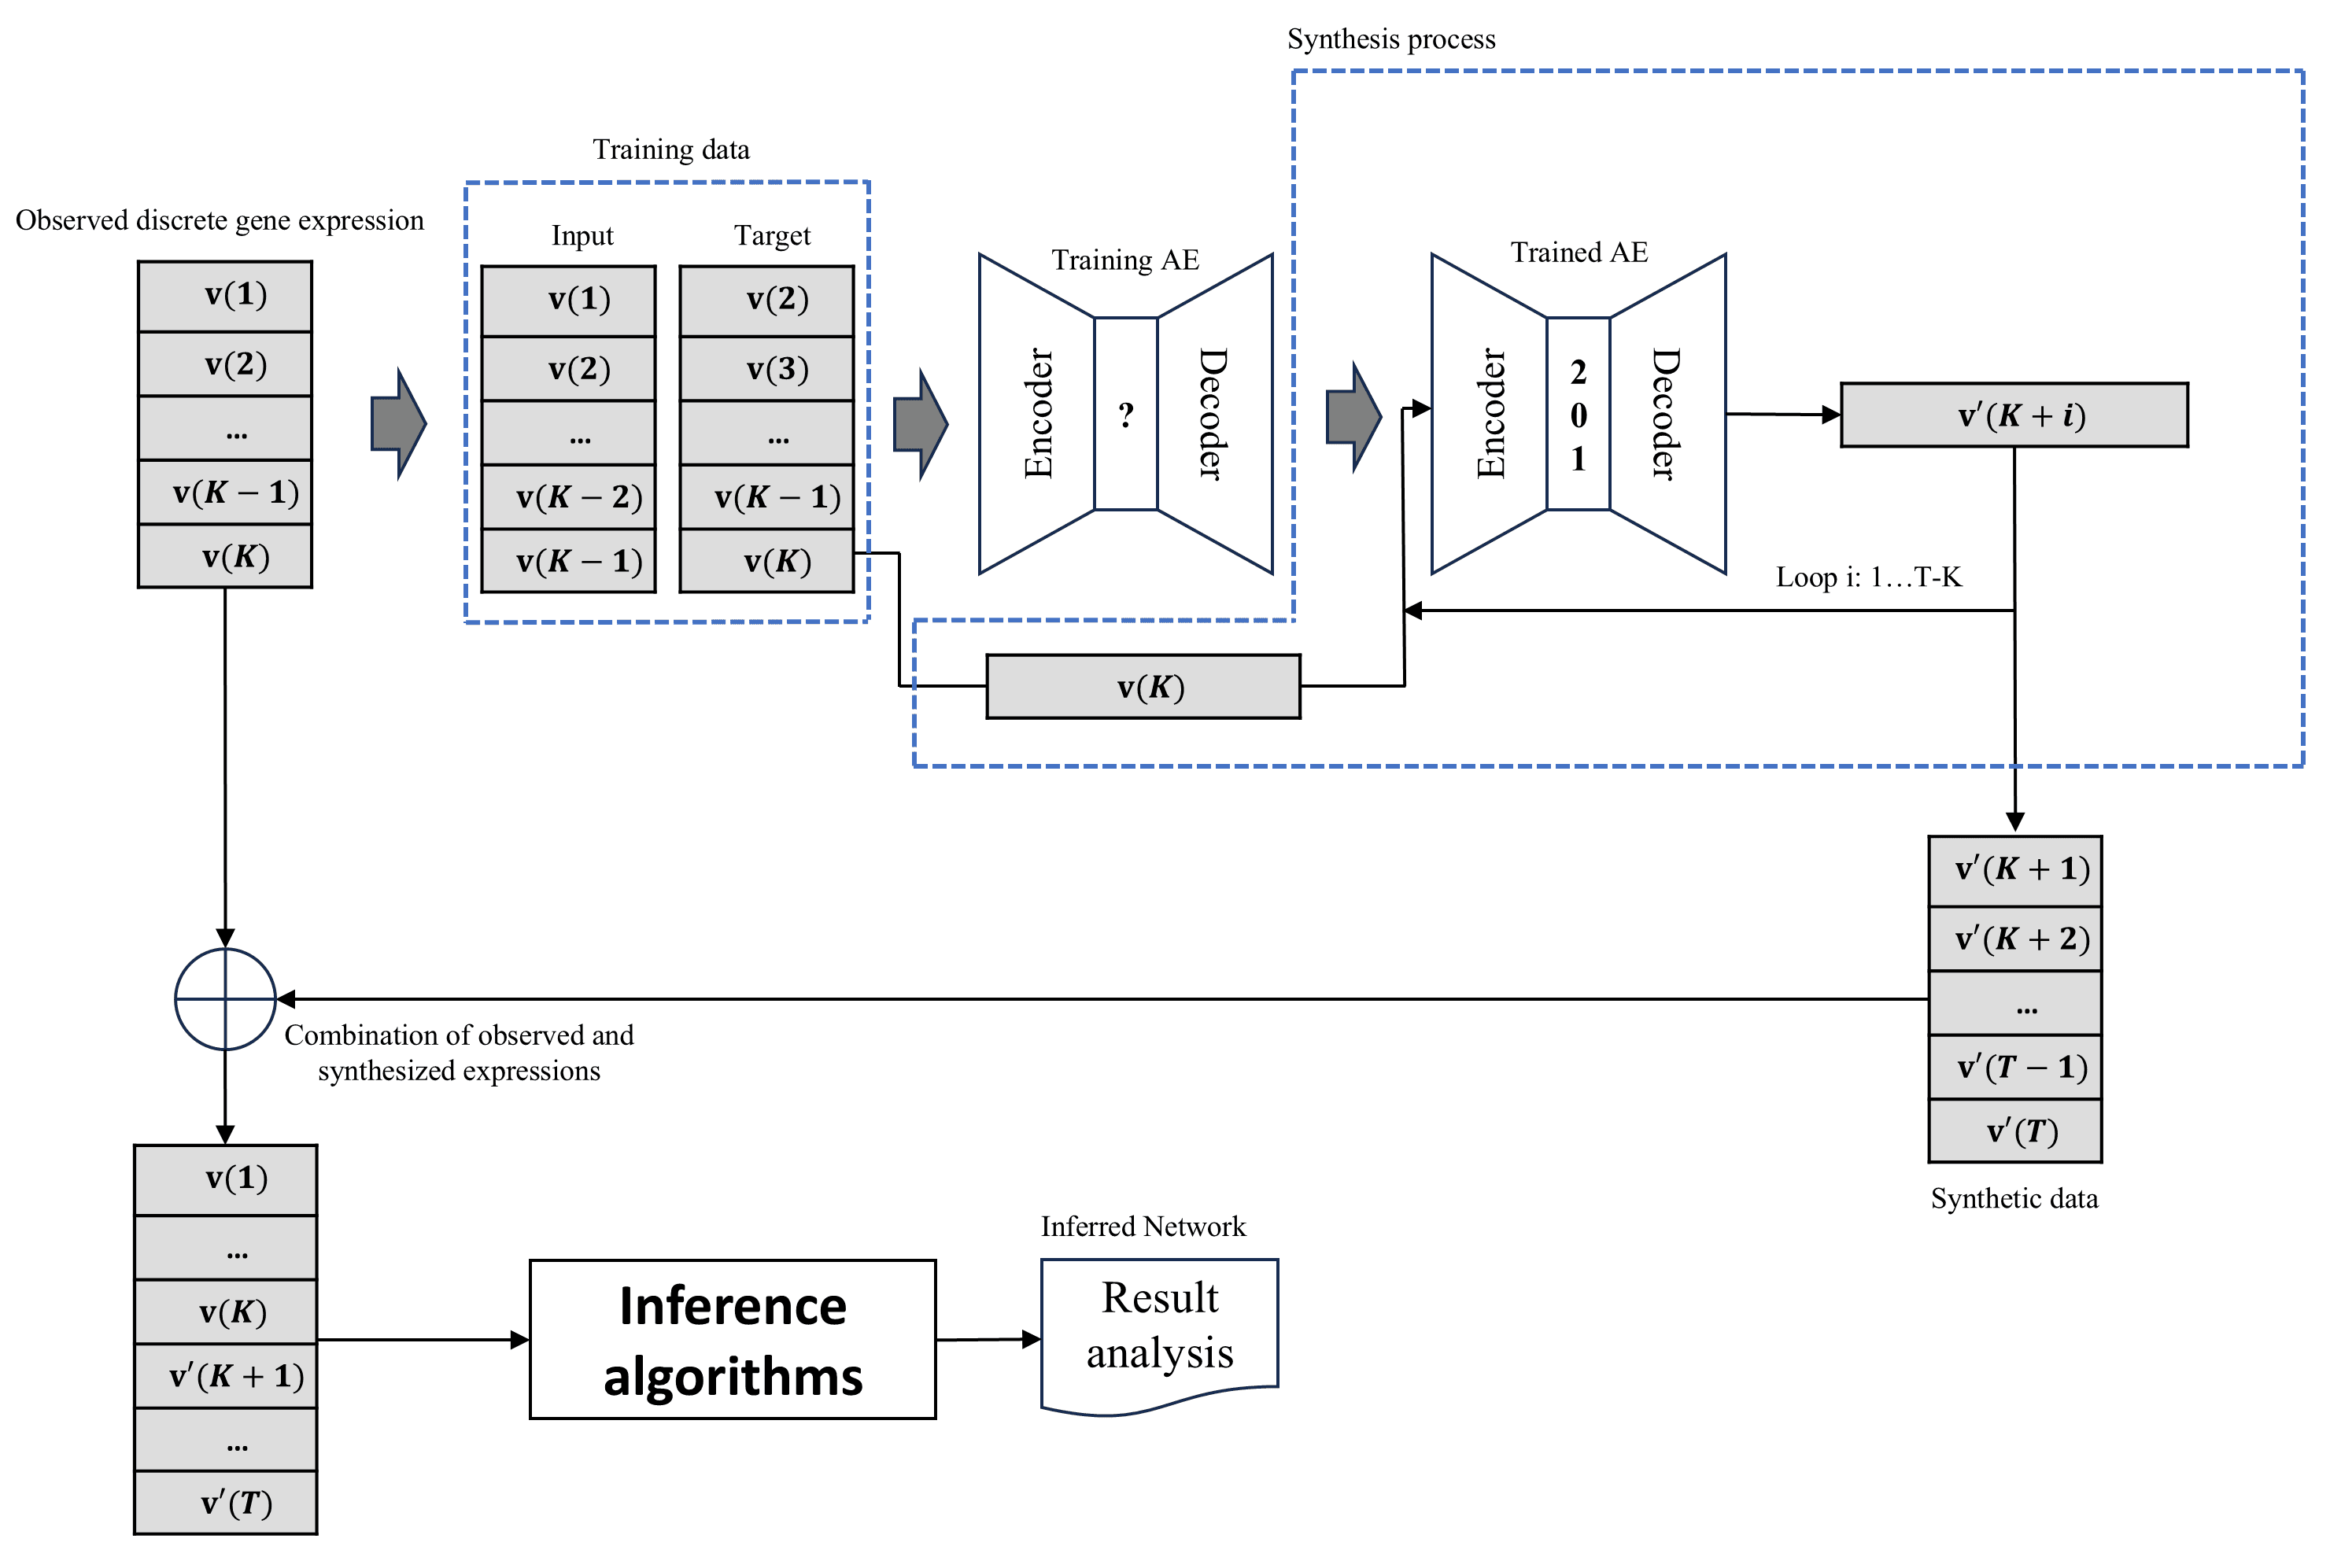
\includegraphics[width=\linewidth]{Figures/chapter4_framework_v9.png}
\decoRule
\caption{The framework of our method. The observed expression data create the input--target matrices, which represent a pair of consecutive expression vectors to train an autoencoder. The trained autoencoder autoregressively synthesizes expression data. The combined data of the observed and synthesized expressions are used as input for the inference algorithms.}
\label{fig:chapter4_framework}
\end{figure}

\subsection{Synthesis of Gene Expression}
The given input data is an observed, discretized gene expression matrix of \(K \times N\) size. Let \(\textbf{v}(t) = [v_1(t), v_2(t),...,v_N(t)]\) be a network state at time step \(t\) represented by a vector of all gene values. Then, the input data are the collection of \(\textbf{v}(t)\) for all observed time steps (\(t=1, 2,~$\dots$, K\)). The observed gene expression matrix is transformed into two \((K-1) \times N\) matrices called the input and target matrices for training the autoencoder. The first and second matrices are the collections of \(\textbf{v}(t)\) ranging from \(t=1\) to \(t=K-1\) and from \(t=2\) to \(t=K\), respectively. This representation can delineate the correlation of gene expression values between two consecutive time steps, enabling the autoencoder to effectively identify the underlying dynamics. After the training process is finished, the autoencoder model can be used to generate unobserved discrete gene expression data after the last observation time step \(K\). At the first iteration of the generation process, \(\textbf{v}(K)\), the network state at the last observation time step is given as an input to the model, and the model produces an output \(\textbf{v$'$}(K+1)\), which is used as an input for the output \(\textbf{v$'$}(K+2)\) and so on. This process is repeated for a desired time step. The structure of the autoencoder is presented in Table~\ref{structure_autoencoder}. We chose the set of parameters that provides the best results, as presented in Table~\ref{training_parameter}. {The model structure and hyperparameters were selected through extensive empirical tuning considering the specific characteristics of biological gene expression data and the demands of network reconstruction tasks. A symmetric three-layer architecture was chosen to provide sufficient capacity for capturing the complex nonlinear relationships commonly observed in gene regulatory networks while avoiding overfitting typically observed in small biological datasets. ReLU activation functions were used in the hidden layers due to their ability to efficiently learn sparse representations. This aligns with the biological assumption that only a subset of genes is co-regulated at a time. In contrast, alternatives like sigmoid and tanh introduced saturation effects and slower convergence. Linear output activation preserves the full dynamic range of gene expression values (between 0 and 2). The learning rate and training epochs were dynamically adjusted to accommodate datasets of varying size and complexity, ensuring stable convergence without sacrificing generalization. These design choices were made to optimize the model’s ability to generate biologically plausible data and support the accurate inference of regulatory interactions.}
\begin{table}[th] 
\caption{The structure of the autoencoder model.\label{structure_autoencoder}}
\begin{tabular}{@{}p{0.75\textwidth} p{0.25\textwidth}@{}} 
\toprule
\textbf{Parameter's Name}	& \textbf{Value}\\
\midrule
Dimension of the input layer & \(N\)\\
Dimension of the output layer & \(N\)\\
Number of hidden layers & 3\\
Number of neurons in the first hidden layer & \(2 \times 
 N\)\\
 %Authors: We changed and confirmed.
Number of neurons in the second hidden layer & 512\\
Number of neurons in the third hidden layer & \(2 \times N\)\\
Activation function in hidden layers & relu\\
Activation function in the output layer & linear\\
\bottomrule
\end{tabular}
\end{table}

\vspace{-10pt}
\begin{table}[th] 
\caption{Parameters of the training.\label{training_parameter}}
\begin{tabular}{@{}p{0.66\textwidth} p{0.33\textwidth}@{}} 
\toprule
\textbf{Parameter's Name}	& \textbf{Value}\\
\midrule
Model optimizer		& Adam	\\
Learning rate & 0.001--0.01 *\\
Loss function & mse\\
Number of epochs & 1000--10,000 *\\
Batch size & 32\\
\bottomrule
\end{tabular}
\noindent{\footnotesize{* The values are different depending on the size of the input network.}}
\end{table}

\subsection{Inference of GRN}
As mentioned in Subsection~\ref{network_inference}, we applied MIDNI to the synthesized discrete gene expression data. Two key parameters are configured for MIDNI in this study: First, the time lag parameter is set to one, that is to say, the expression of a regulator gene at time step \(t\) influences the expression of its target gene at time step \((t + 1)\). The time lag accounts for the inherent delays in biological processes, such as transcription, translation, and the diffusion of regulatory molecules, which are essential for accurately capturing the dynamic nature of gene regulatory interactions. Second, the maximum number of regulators is set to five. This constraint reduces the computational complexity of the network inference process while maintaining biological relevance such that most genes are regulated by a relatively small number of key regulators in real biological systems.

\section{Experimental Results}
\subsection{Experiment Setup}
To comprehensively evaluate the performance and robustness of our proposed method, we conducted experiments on synthetic datasets representing GRNs of two different network sizes \(N = 50\) and \(N = 100\). These sizes were chosen to reflect small-to-intermediate complex biological systems, allowing us to examine the scalability of our method under different conditions.
For each network size, we generated 10 structurally distinct ground truth networks using the Barabási--Albert (BA) model \parencite{Barabasi2006}, which is a widely used generative model that captures the scale-free properties commonly observed in real-world biological networks. This resulted in a total of 20 unique ground truth networks used in our experiments.
For each ground truth network, we simulated discretized gene expression data over \(K\) observed time steps using a dynamic model outlined in Algorithms ~\ref{alg:random_update_function} and ~\ref{alg:random_gene_exression} (see Appendix ~\ref{AppendixB}). These simulated time-series datasets serve as the foundation for evaluating our method's ability to infer network structure from temporal gene expression patterns. Two levels of discretization were considered to reflect different degrees of resolution in experimental measurements, namely binary (two states: 0 or 1) and ternary (three states: 0, 1, or 2). This allowed us to assess the method's sensitivity and effectiveness across datasets with varying levels of granularity.
Our method takes the observed gene expression data over the initial \(K\) time steps as input and synthesizes the gene expression values for the remaining \((T - K)\) time steps, where the total length of the time-series is fixed at \(T = 100\). The ability to generate synthetic future data is a critical component of our approach, as it allows us to enrich the dataset and potentially improve inference accuracy, especially in cases where only a limited number of observations are available.
To systematically investigate the influence of the number of observed time steps on inference performance, we varied \(K\) from 10 to 90 in increments of 10. This setup enables us to explore how the quantity of available temporal data affects both the quality of synthetic data generation and the subsequent network inference.
We applied the network inference algorithm, MIDNI, to both the original and synthesized datasets. The inferred networks were then compared against the corresponding ground truth networks using the evaluation metrics explained in Section ~\ref{sub:metrics}. Performance was analyzed separately for datasets discretized into ternary levels (see Figure~\ref{chapter4_triple_performance}) and binary levels (see Figure~\ref{fig:chapter4_bool_performance}). Comprehensive results are provided in Tables ~\ref{tab:performance-latest} and ~\ref{tab:performance-updated-latest} (see Appendix ~\ref{AppendixC}). These comparisons provide insight into how well our method reconstructs the underlying network structure under different data conditions and discretization schemes.


\begin{figure}[th]
\centering
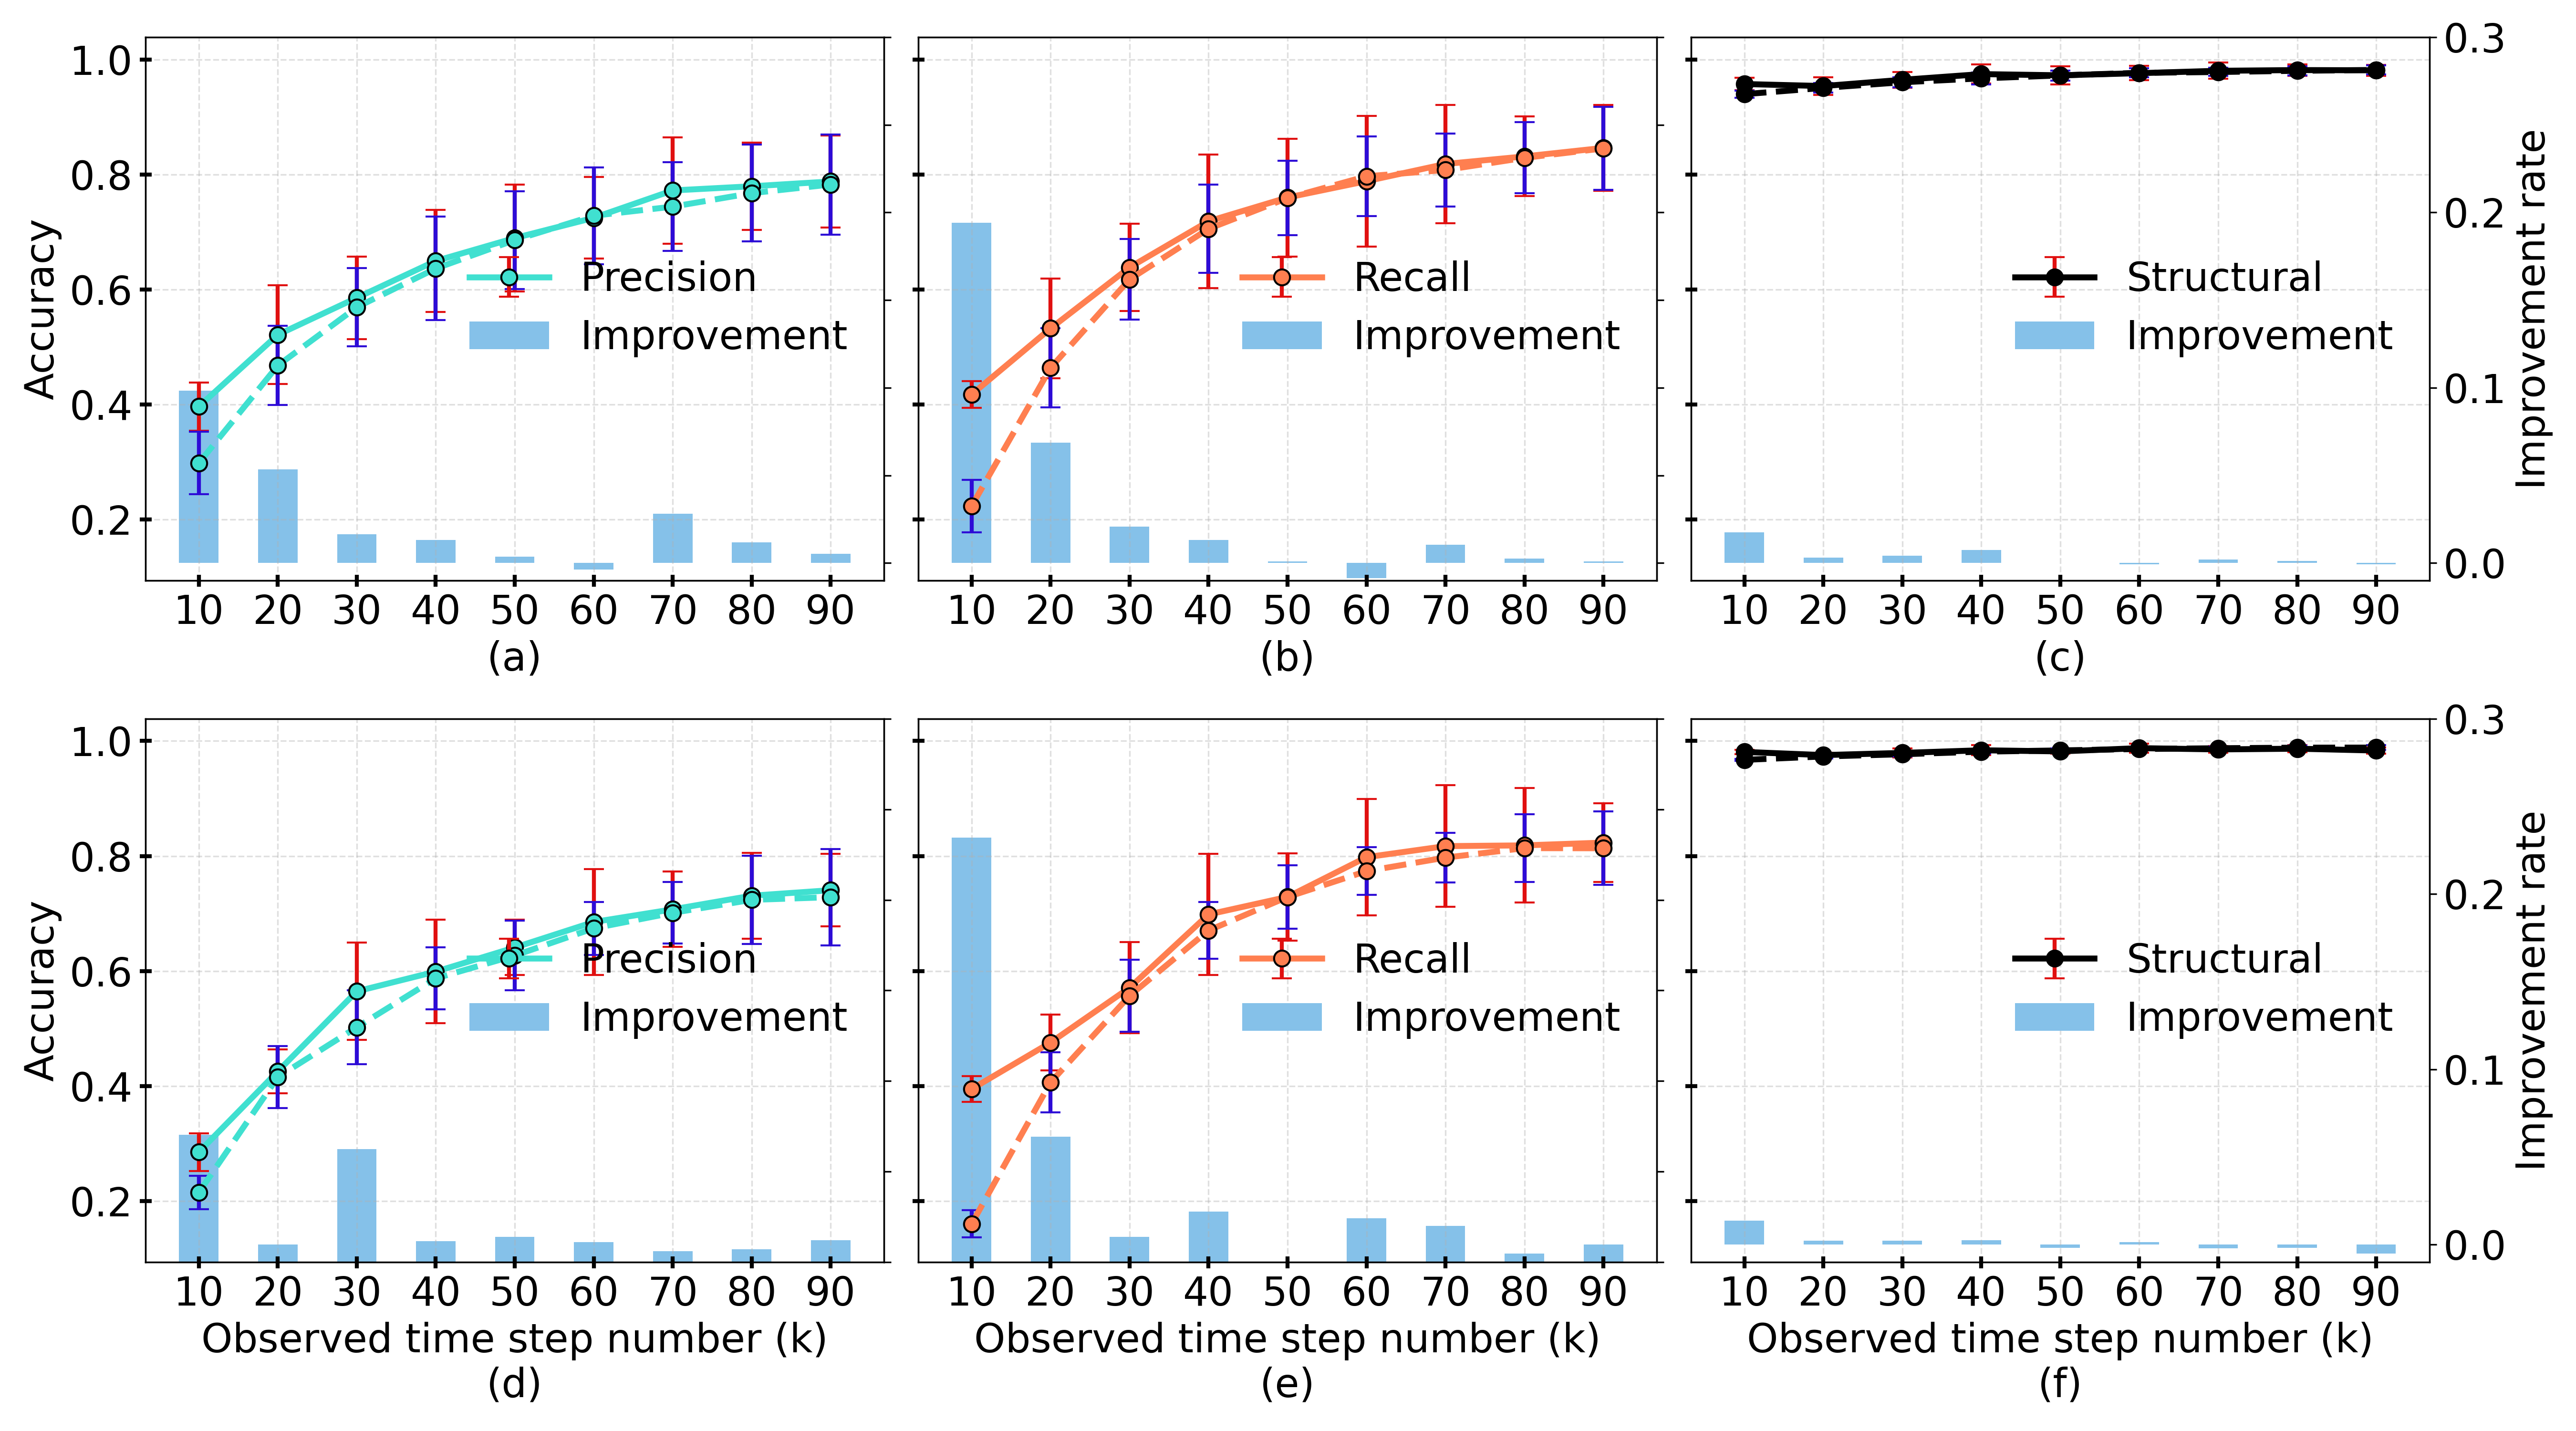
\includegraphics[width=\linewidth]{Figures/chapter4_triple_performance.png}
\decoRule
\caption{Results of precision, recall, and structural accuracy on the multi-level discretization dataset. (\textbf{a}--\textbf{c}). Results for the network with \(|V|=50\). (\textbf{d}--\textbf{f}).Results for the network with \(|V|=100\). The Y-axis denotes the performance metrics, and the X-axis indicates the number of observed time steps in the original gene expression data. For the synthesized dataset, gene expression data are generated for \((100-K)\) time steps. Solid and dashed lines represent the results based on the synthesized and the original dataset, respectively. Each point and error bar indicates the average value and the standard deviation, respectively, over 10 random networks. The bar charts show the performance improvement of the synthesized dataset over the original dataset.}
\label{chapter4_triple_performance}
\end{figure}

\vspace{-10pt}

\begin{figure}[th]
\centering
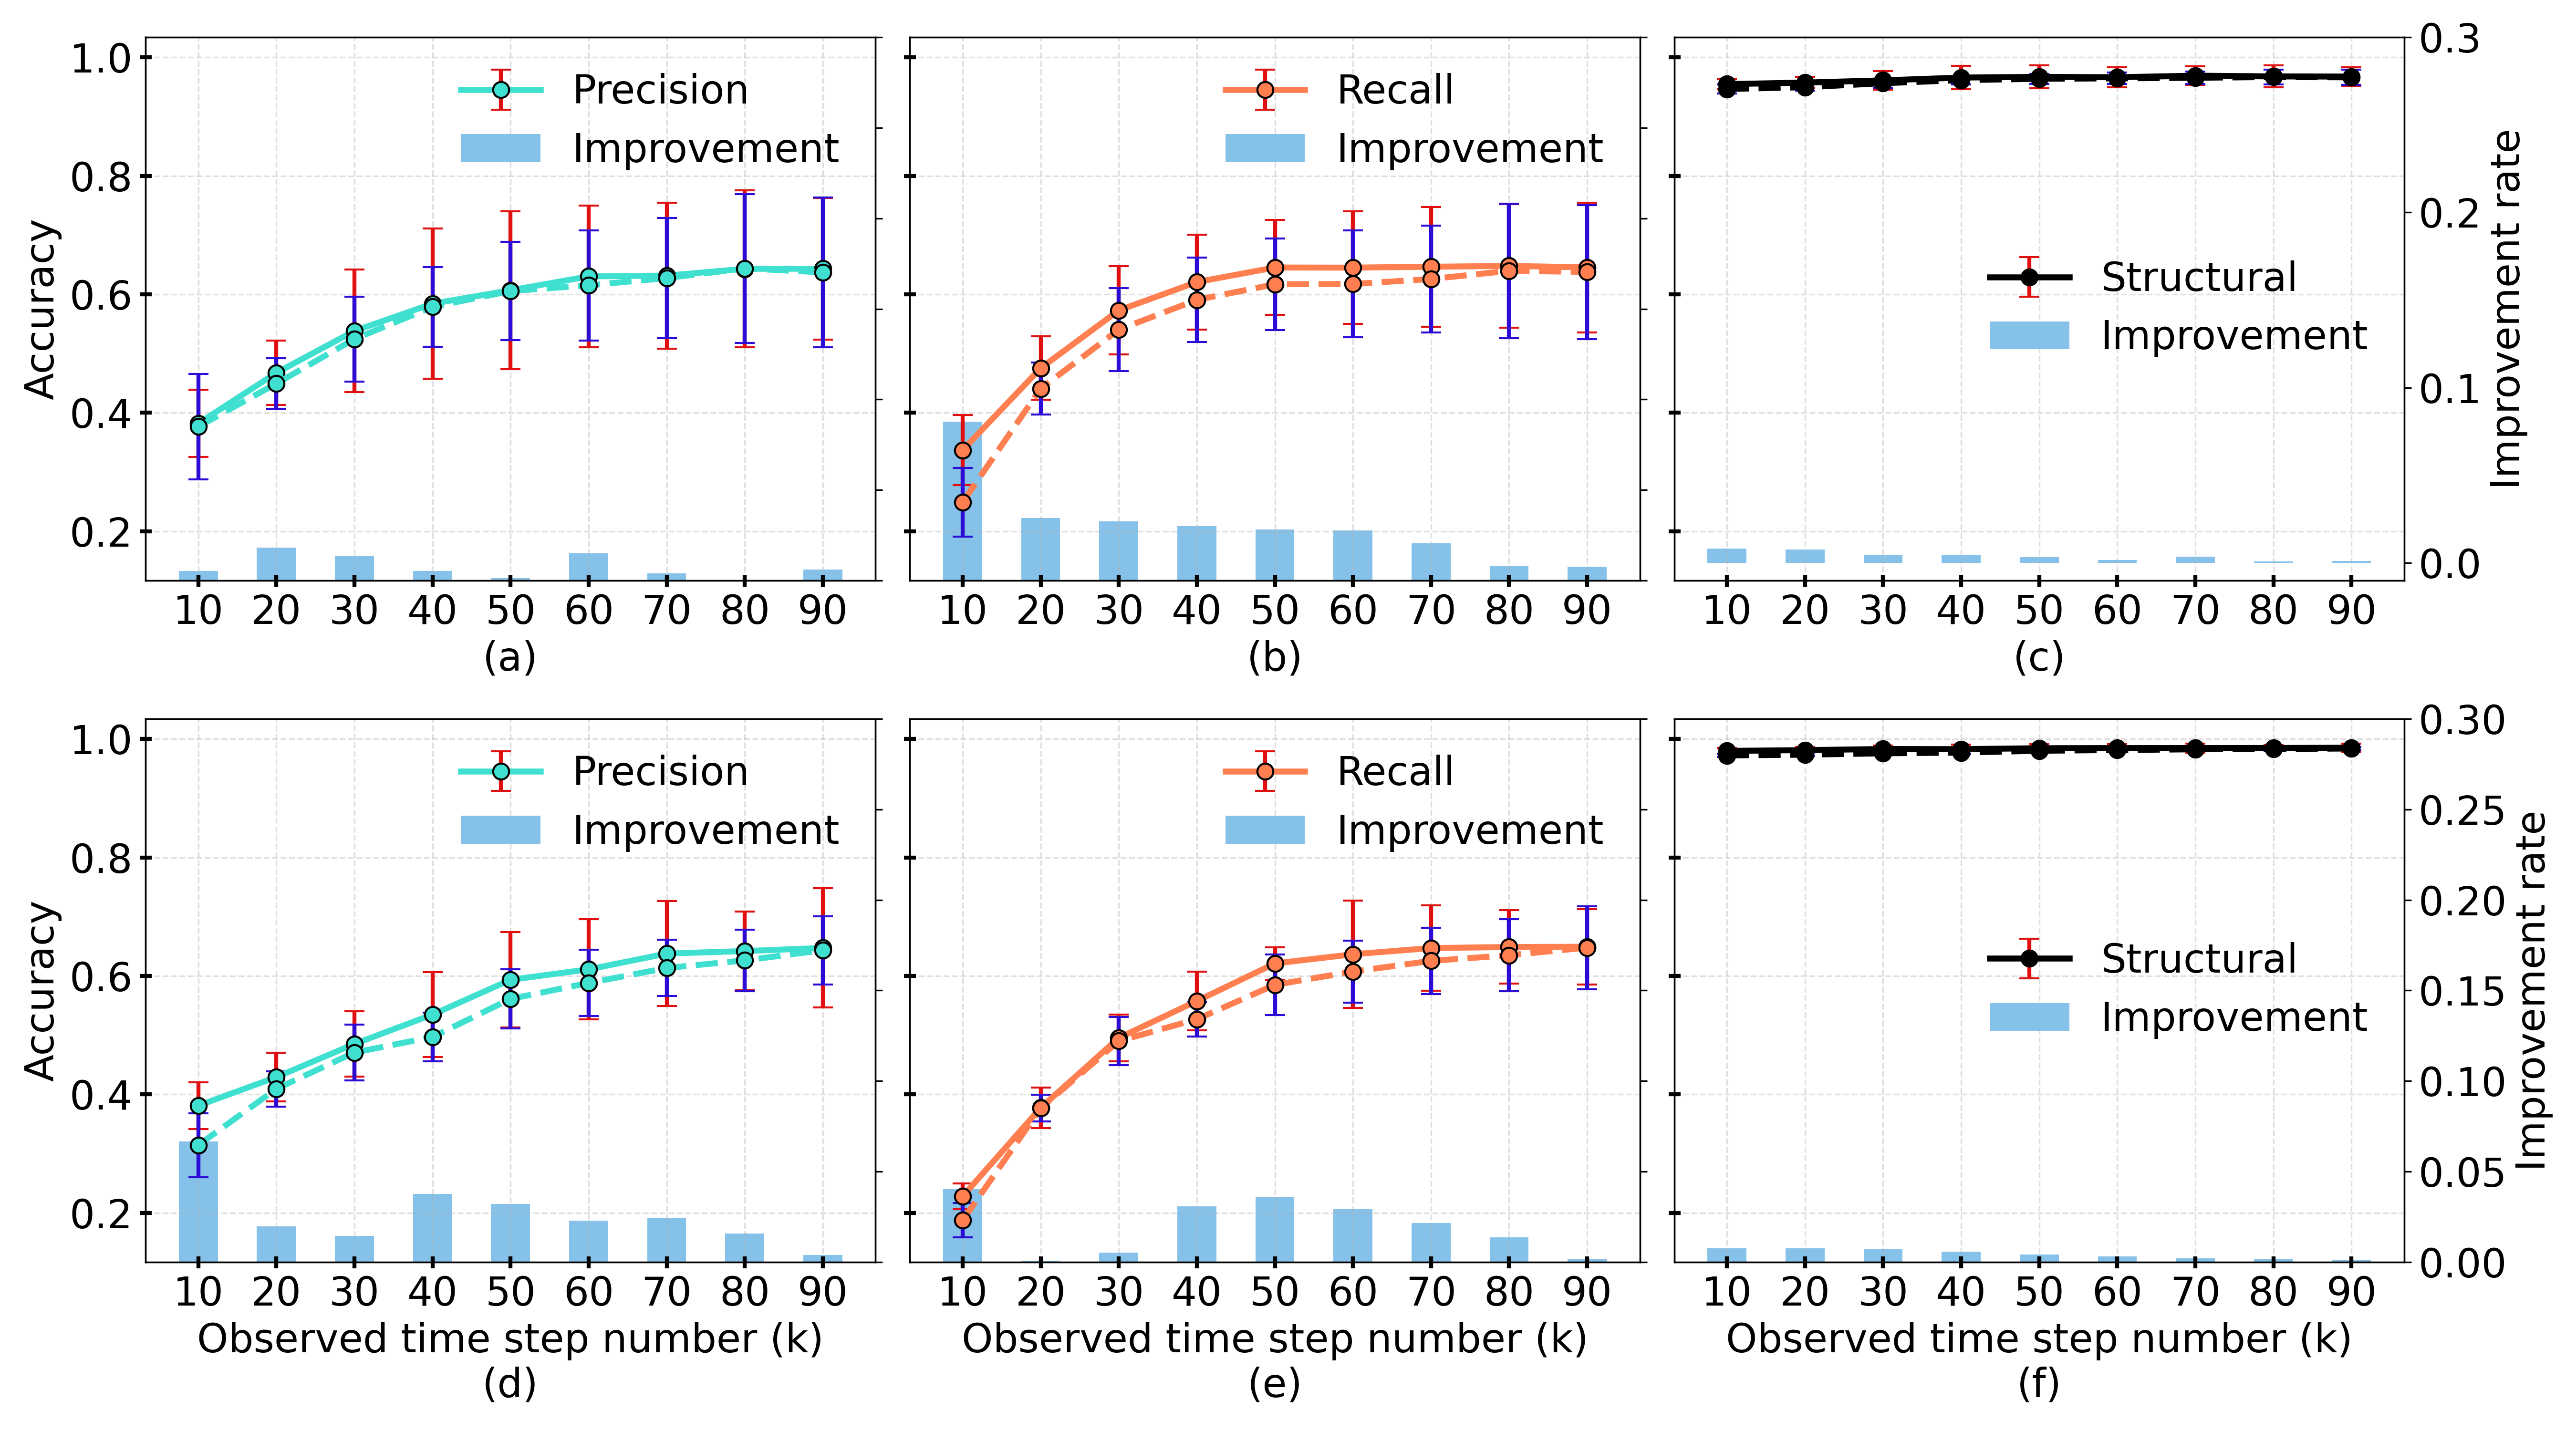
\includegraphics[width=\linewidth]{Figures/chapter4_bool_performance.png}
\decoRule
\caption{Results of precision, recall, and structural accuracy on the Boolean discretization dataset. (\textbf{a}--\textbf{c}) Results for the network with \(|V|=50\). (\textbf{d}--\textbf{f}) Results for the network with \(|V|=100\). The Y-axis denotes the performance metrics, and the X-axis indicates the number of observed time steps in the original gene expression data. For the synthesized dataset, gene expression data are generated for \((100-K)\) time steps. Solid and dashed lines represent the results based on the synthesized and the original dataset, respectively. Each point and error bar indicates the average value and the standard deviation, respectively, over 10 random networks. The bar charts show the performance improvement of the synthesized dataset over the original dataset.}
\label{fig:chapter4_bool_performance}
\end{figure}

\subsection{Results of Structural Performance}
 As shown in Figure~\ref{chapter4_triple_performance}a (see Table ~\ref{tab:performance-latest} in Appendix ~\ref{AppendixC} for details), the precision values of the networks inferred based on the original data (dashed line) and the synthetic data (solid line) continuously increase as the observed time steps (\(K\)) increase in the networks with \(|V|=50\). This is because the more expression data used for the inference algorithm, the higher the inference performance. The precision improvement by the use of the synthetic data was observed in all \(K\) values except for \(K=60\) and 90. In addition, we can observe a similar trend with respect to the recall performance (Figure~\ref{chapter4_triple_performance}b). In particular, the degree of the performance improvement at \(K=10\) was significantly larger. These observations indicate that the precision improvement by the synthetic data is not by reducing the number of positive predictions of interactions but by predicting the true positive interactions more accurately. Although the synthetic data also improved the structural accuracy, the improvement was not significant (Figure~\ref{chapter4_triple_performance}c). This is because the number of true negatives is much larger than that of true positives. We note that these findings were consistently observed in the networks with a larger network size (\(|V|=100\)) (Figure~\ref{chapter4_triple_performance}d--f). Taken together, our synthetic approach can be considerably useful when the observation time of the gene expression is limited in the real experimental environment. \par
We also investigated our method with respect to the Boolean networks, as shown in Figure~\ref{fig:chapter4_bool_performance} (see Table ~\ref{tab:performance-updated-latest} in Appendix ~\ref{AppendixC} for details). As in the ternary network results, we can observe the performance improvement of precision, recall, and structural accuracy in most cases. This means that our method is also effective in the Boolean network models. It is interesting that the recall improvement by our method was relatively larger on average than the precision improvement in the case of \(|V|=50\), whereas the latter was relatively larger than the first in the case of \(|V|=100\). This is because the MIDNI algorithm cannot control the number of positive predictions. However, we note that there is no negative influence on any performance measure. It is also interesting that the performance improvement does not increase as the observation time step \(K\) increases. For example, the precision was highest when \(K\) is 60 and 50 in the networks of \(|V|=50\) and \(|V|=100\), respectively (Figure~\ref{fig:chapter4_bool_performance}a,d), and the recall was highest at \(K=70\) in the networks of \(|V|=100\) (Figure~\ref{fig:chapter4_bool_performance}e). These results mean that the desirable number of observation time steps is dependent on the degree of discretization levels. \par
\subsection{Results of Dynamic Accuracy}
We also evaluated the dynamic accuracy of both the networks inferred from the original and the synthetic data on the multi-level discretization dataset (Figure~\ref{dynamic_triple}) and on the Boolean discretization dataset (Figure~\ref{dynamic_bool}). Contrary to precision or recall metrics, the dynamic accuracy tends to decrease as the number of time steps increases. We believe this is due to the increase in the number of data samples to be fitted by the inferred network. {Moreover, the incorporation of additional time points may introduce deviations from the patterns already learned by the model, particularly if the new data include noise, nonlinear dynamics, or previously unobserved system behaviors}. In addition, the dynamic accuracy of the synthetic data-driven networks is inferior to that of the original data-driven networks in most cases. We note that the latter is investigated over \(K\) time steps, whereas the former is investigated over \(T\) time steps, which is longer than \(K\). Considering this difference between the examination time steps, the performance difference in terms of the dynamics accuracy may not be considerably significant.

\begin{figure}[th]
\centering
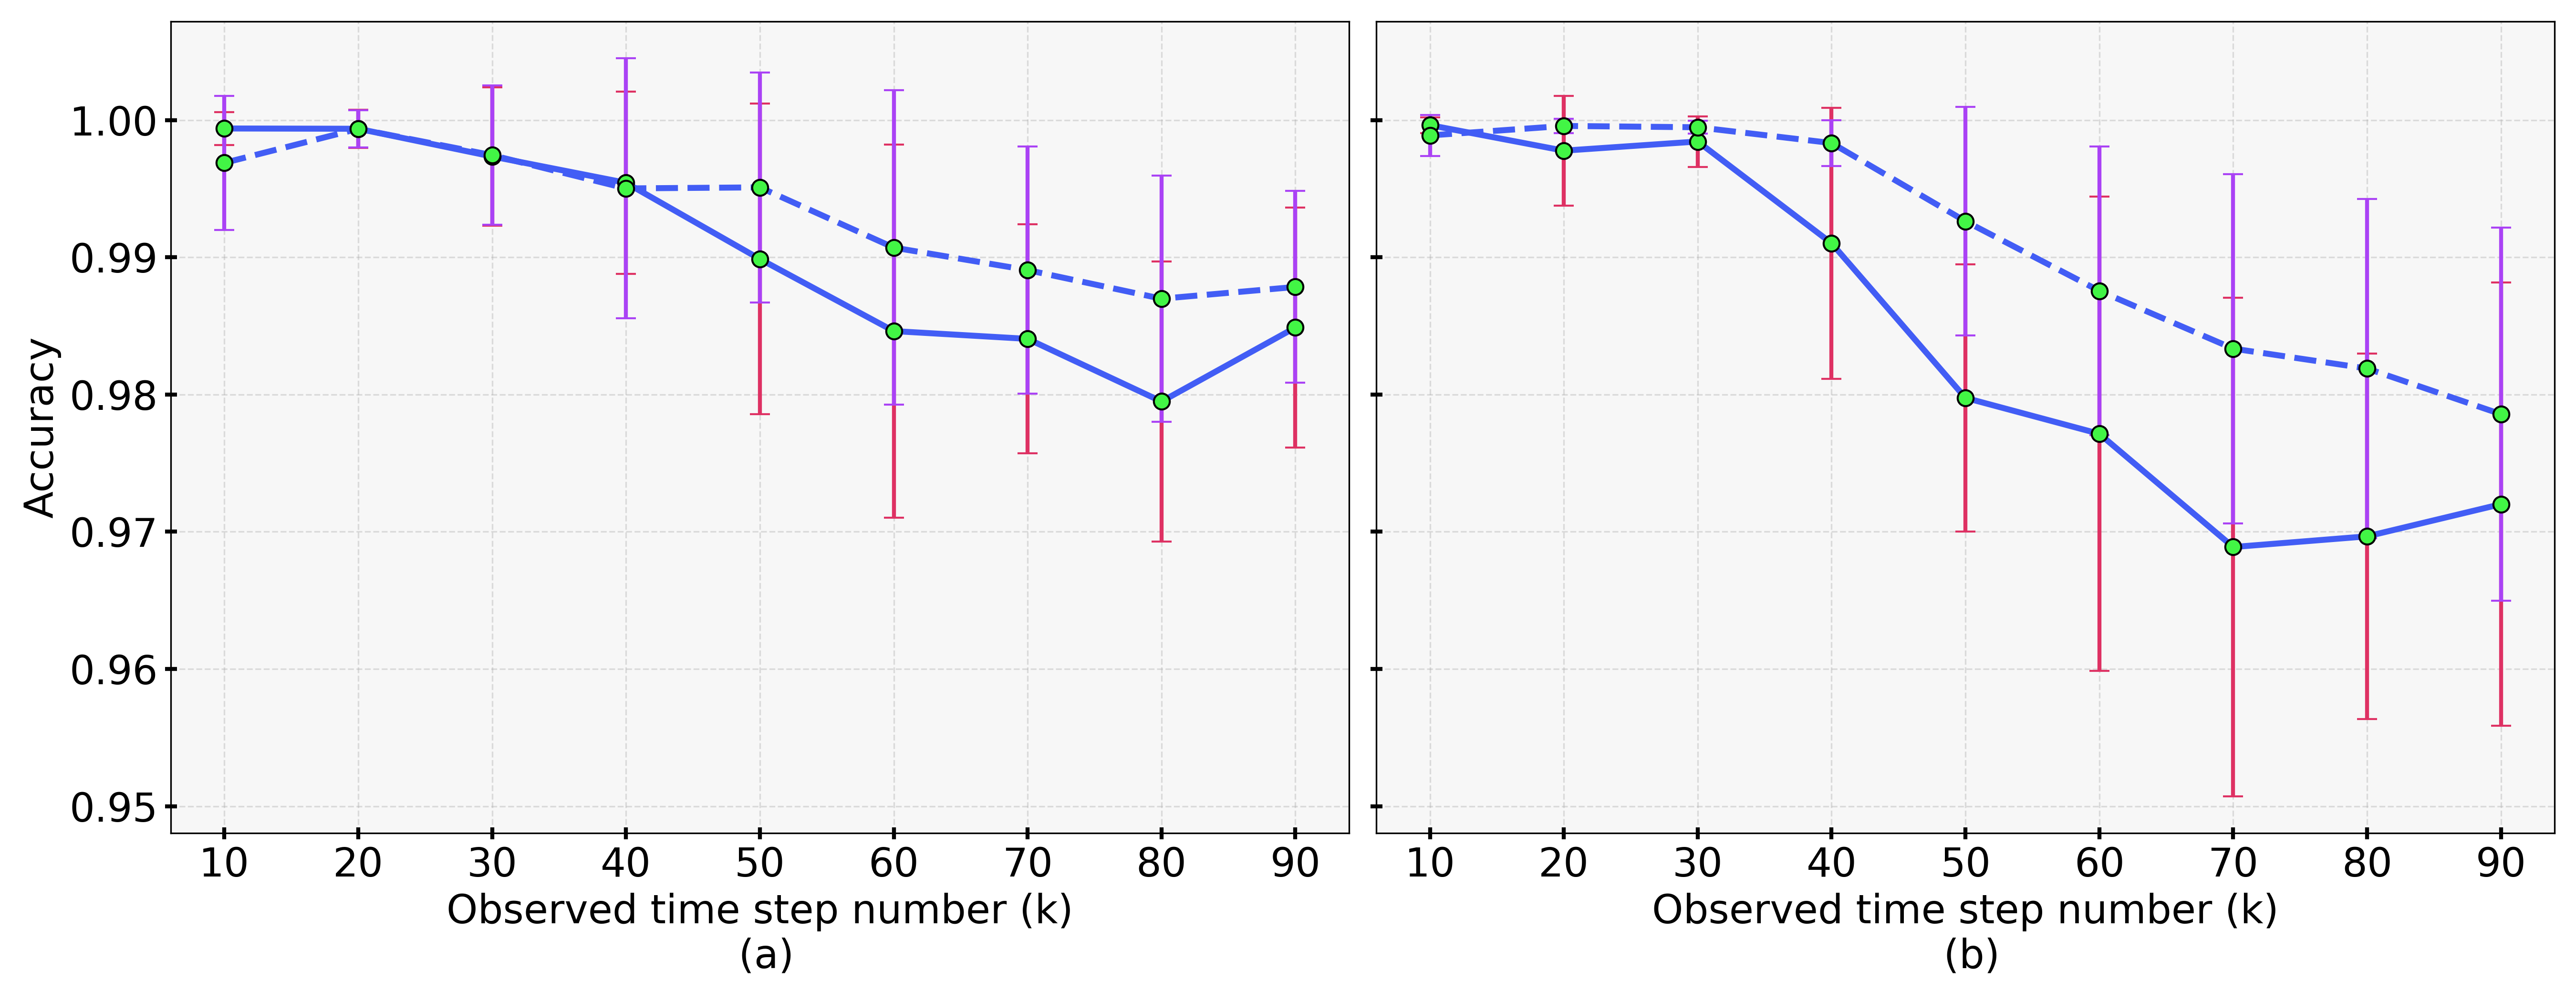
\includegraphics[width=\linewidth]{Figures/chapter4_triple_dynamics.png}
\decoRule
\caption{Comparison results of dynamic accuracy on the multi-level discretization dataset. (\textbf{a}) Networks of \(|V|=50\). (\textbf{b}) Networks of \(|V|=100\). The Y-axis denotes the dynamic accuracy, and the X-axis indicates the number of observed time steps. The dashed and solid lines represent the results of the networks inferred from the original and the synthetic expression data, respectively.}
\label{dynamic_triple}
\end{figure}

\vspace{-8pt}

\begin{figure}[th]
\centering
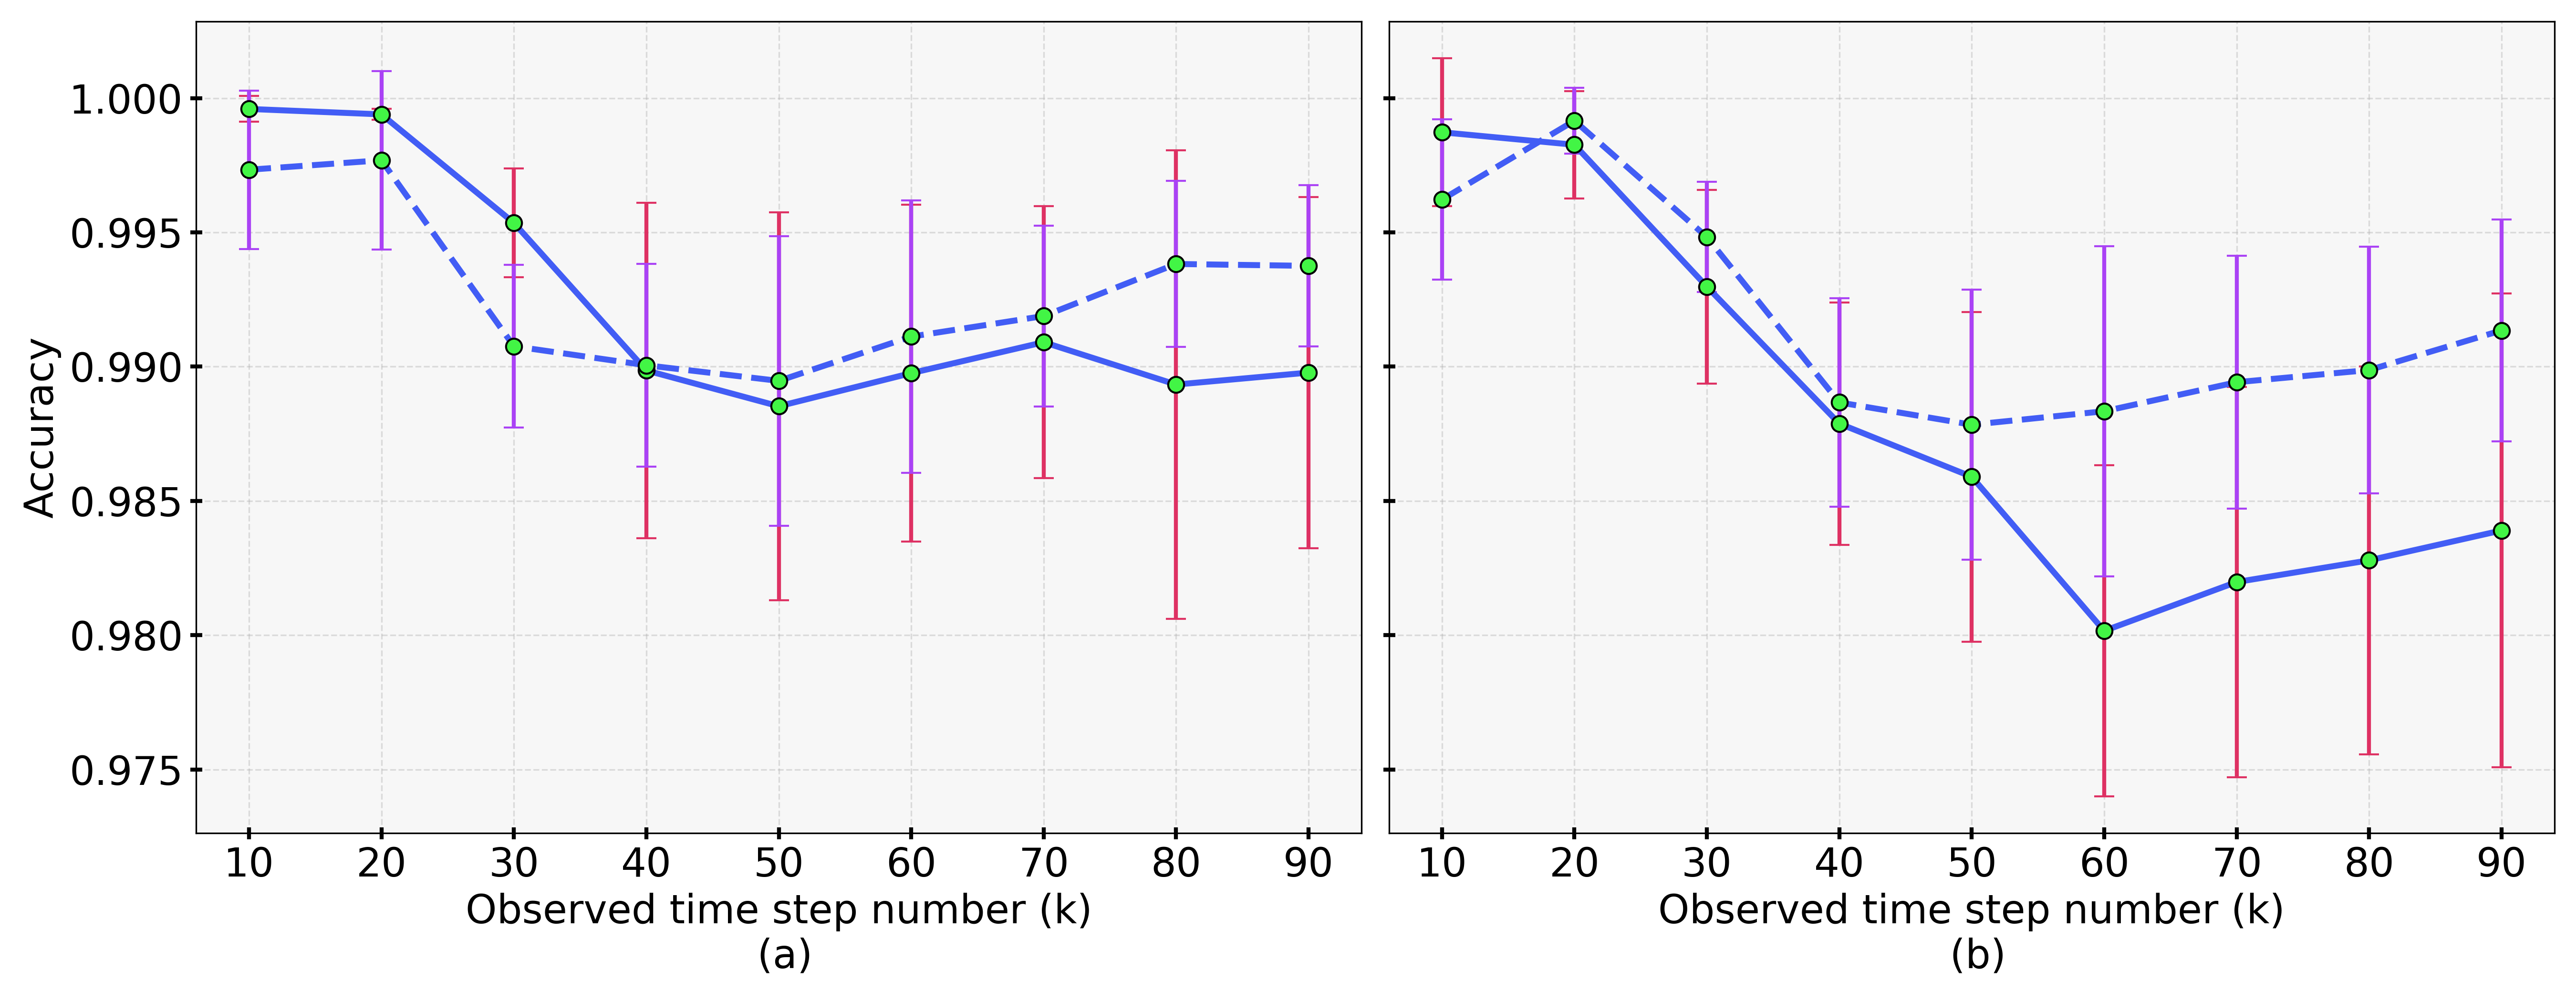
\includegraphics[width=\linewidth]{Figures/chapter4_bool_dynamics.png}
\decoRule
\caption{Comparison results of the dynamic accuracy on the Boolean discretization dataset. (\textbf{a})~Networks of \(|V|=50\). (\textbf{b}) Networks of \(|V|=100\). The Y-axis denotes the dynamic accuracy, and the X-axis indicates the number of observed time steps. The dashed and solid lines represent the results of the networks inferred from the original and the synthetic expression data, respectively.}
\label{dynamic_bool}
\end{figure}

\subsection{Results of Similarity of Synthesized Expressions}
{The autoencoder can generate the gene expression data differently whenever it is executed. To investigate how much the synthesized data are varied, we first created a random ground truth network with \(N=100\) and generated an original ternary gene expression with \(K\) time steps ranging from 10 to 90 (see Algorithm ~\ref{alg:random_gene_exression} in Appendix ~\ref{AppendixB}). For each \(K\), we trained an autoencoder using the original gene expression and generated three different synthetic gene expressions for later \(=T-K\) time steps. For three pairs of the gene expression matrices of \(T \times N\) size, we investigated the similarity matrix, where the white and the black dots represent whether the corresponding gene expression values in the pair matrices are identical or not, respectively (Figure~\ref{distance}). As shown in the figure, the synthesized gene expressions are significantly different from each other. However, the inference performance based on these synthetic data is not significantly different. In other words, the autoencoder model produces diverse synthesized expressions but induces stable performance.}

\begin{figure}[th]
\centering
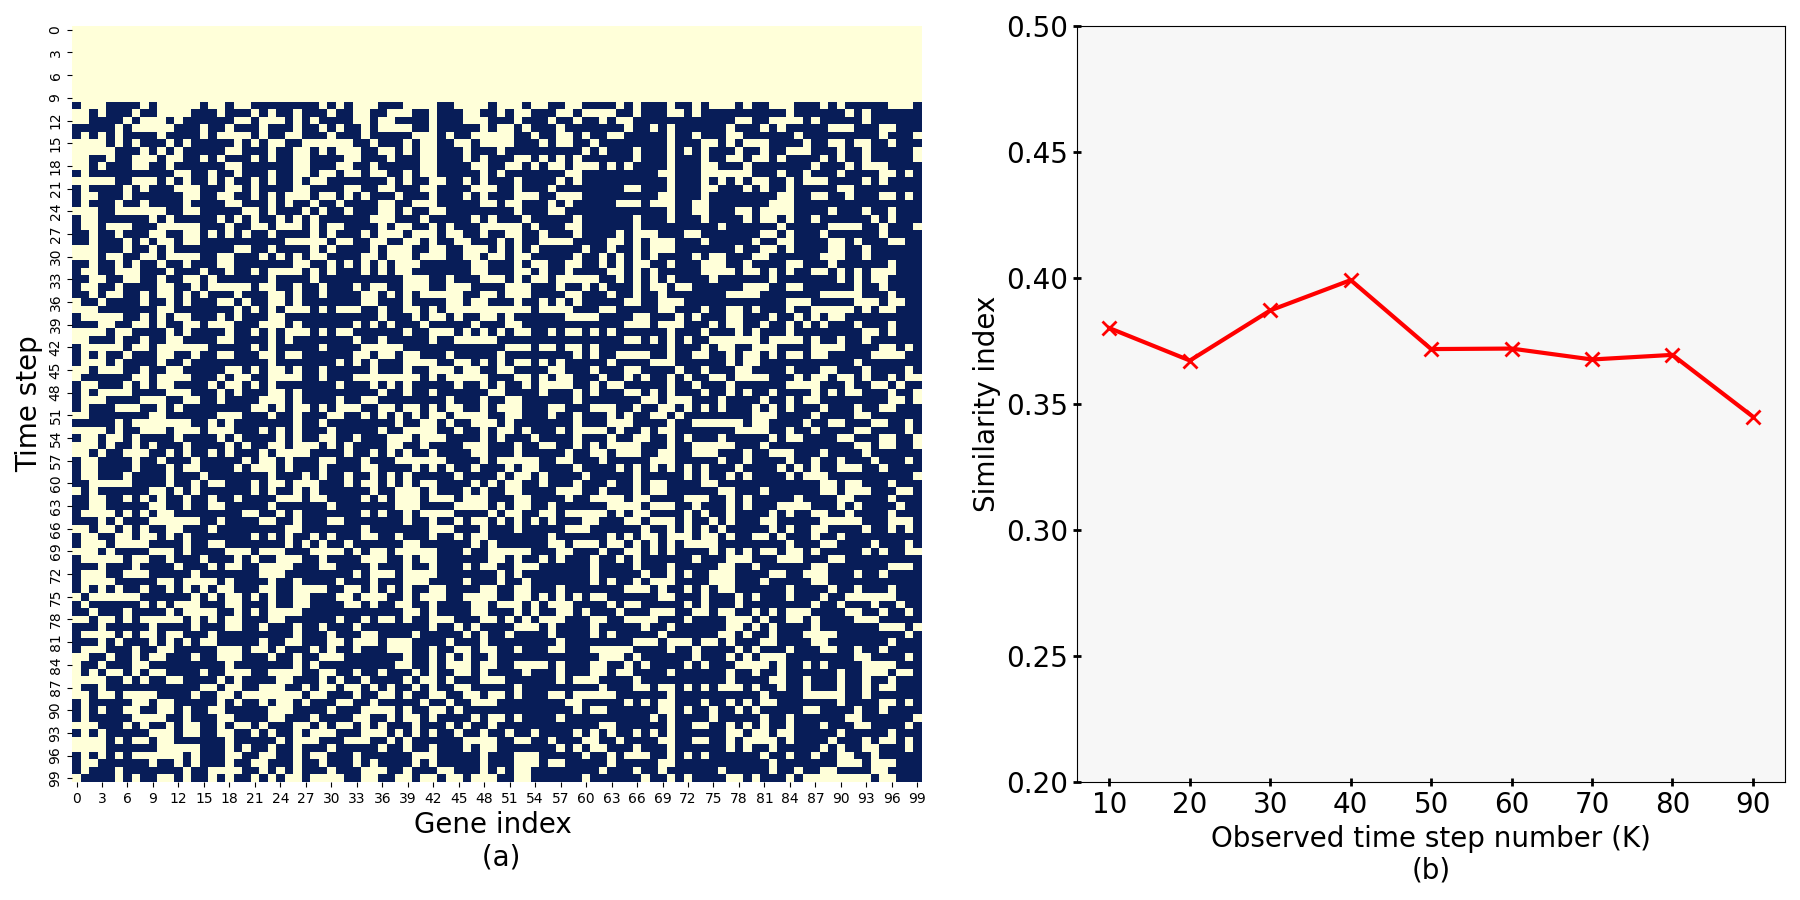
\includegraphics[width=\linewidth]{Figures/chapter4_networks_distance_v2.png}
\decoRule
\caption{Similarity matrix between the synthesized gene expression data. (\textbf{a}) An example of a similarity matrix between a pair of synthesized gene expression data values when \(K\) equals 10. The white or black dot indicates that the corresponding gene values between two expression data values are identical or not, respectively. (\textbf{b}) Change in the mean similarity index against the time step number (\(K\)). For each \(K\) from 10 to 90, three pairs of synthesized gene expression data values were used to compute the mean similarity index. The Y-axis denotes the similarity index, defined as the rate of the number of identical dots over the total number of dots in the gene expression matrix. The X-axis corresponds to the number of observed time steps \(K\). }
\label{distance}
\end{figure}

\section{Discussion and Conclusions}
In this study, we used an autoencoder model to synthesize gene expression data to overcome data scarcity problems in reverse engineering. Specifically, it produces additional time-series expression data to complement the observed gene expression data. The synthesized gene expression data were assessed using an inference algorithm. The experimental results demonstrated that the inference performance using synthetic gene expression was consistently higher than that using only the observed gene expression. This finding substantiates the effectiveness of the proposed model as a valuable tool for addressing network inference problems, particularly when there is a limitation in obtaining gene expression data of a sufficiently long observation time. \par
{Furthermore, as gene expression data inherently possess structural relationships among genes, future work could explore the integration of graph representation learning techniques as a complementary or alternative approach. These methods are well-suited for modeling structured biological systems and may improve the quality of synthetic data or enhance network inference performance by capturing complex topological patterns in gene regulatory networks \parencite{Chen2020, Li2024}. Another future study could be to extend the current framework based primarily on discretized gene expression data to operate directly on continuous-valued datasets. The reliance on discretization introduces variability due to method-specific assumptions, potentially affecting inference outcomes. Developing a discretization-free approach would increase the generalizability of the method. Additionally, integrating more advanced generative models such as GANs may further improve the diversity and biological realism of the synthesized data. Finally, a comprehensive validation of real-world biological datasets will be essential to evaluate the robustness and practical utility of the proposed method across diverse application scenarios, including rare disease modeling and temporal transcriptomic analyses}.


